\documentclass[11pt]{article}
\usepackage{geometry}
\usepackage{lipsum}
\usepackage{multicol}
\usepackage{enumitem}
\usepackage{fancyhdr}
\usepackage[english]{babel}
\usepackage[sc]{mathpazo}                   
\usepackage{graphics}

\usepackage[%  
    colorlinks=true,
    pdfborder={0 0 0},
    linkcolor=red
]{hyperref}

\setlist[itemize]{noitemsep, topsep=0pt}
\setlist[enumerate]{noitemsep, topsep=0pt}

\pagestyle{fancy}
\renewcommand{\headrulewidth}{0pt}
\newcommand{\bb}[1]{\textbf{#1}}


\graphicspath{ {./imgs/} }

\fancyhead[L]{CSCI 545: Introduction to Robotics}
\fancyhead[R]{Fall 2019}

\title{Lecture 17: \it{Motion Planning I}}
\author{Scribe:  \it{Duong Le, Keyu Han, Baiyu Huang, Seunghee Yoon}}
\date{}


\begin{document}
\maketitle
\thispagestyle{fancy}
\section{Complete Motion Planning}
\subsection{Cell Decompose}
\subsection{Visibility Graph}
\section{Sampling-based Motion Planning}
Sampling-based motion planning is not complete: not guarantee to find a solution when one exists. However, as the number of samples goes to infinity, there is a strong guarantee that it can find a solution.\\
There are 2 types of sample-based planning algorithms:\\
\begin{multicols*}{2}
\textbf{\underline{Multiple Query Algorithm}}
\begin{itemize}
\item Roadmap is built beforehand. Then it can be used multiple times for different queries.
\item Query is fast since roadmap is already generated.
\item Keeping roadmap all the time is expensive.
\item Can only deal with static environment - has to rebuild the roadmap when environment changed.
\end{itemize}
\vfill\null
\columnbreak
\textbf{\underline{Single Query Algorithm}}
\begin{itemize}
\item No roadmap is built beforehand. Find a path from start to goal then finish
\item Query is slower.\\
\item No saved roadmap - better memory \\
\item Can deal with dynamic environment 
\end{itemize}
\end{multicols*}

\subsection{Probabilistic Road Map (PRM)}
Probabilistic Roadmap (PRM) is a multi-query algorithm.\\
There are 2 steps:
\begin{enumerate}
\item Preprocessing state: build roadmap
\item Query state: search roadmap given start and goal
\end{enumerate}

\subsubsection{Roadmap Construction}
\begin{figure}[h]
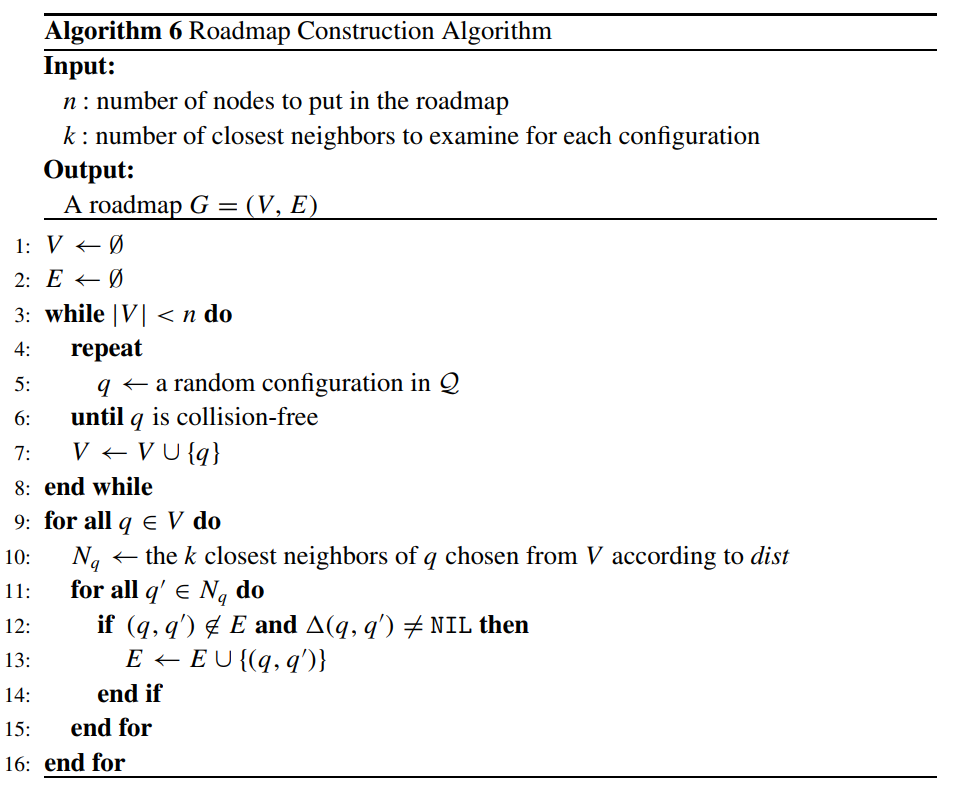
\includegraphics{PRM}
\centering
\caption{Roadmap Construction Algorithm}
\label{fig:roadmap_alg}
\end{figure}
Let $\Delta(q, q')$ be a function that returns either a collision-free path from q to q' or NIL if it cannot find such a path. There are many algorithms can be used for $\Delta$. For example, if we want to check whether there is a straight-line path from q to q, we can use binary search to check for collision.\\
Figure \ref{fig:roadmap_alg} shows an algorithm to construct a roadmap:
\begin{itemize}
\item Line (1) and (2): Initialize graph $G=(V,E)$ to be empty.
\item Line (3) to (8): describes sampling process: keep sampling to get $n$ numbers of collision-free samples.
\item Line (9) to end: describes process to build roadmap from $n$ samples: for every sample node $q\in V$, create a set $N_q$ of $k$ closest neighbors. Then from every $q' \in N_q$, whenever function $\Delta(q, q')$ succeeds to compute a collision-free path from $q$ to $q'$, the edge $(q,q')$ is added to $E$. Figure \ref{fig:roadmap_example} shows an example of roadmap using $\Delta$ as straight-line planner
\end{itemize}

\begin{figure}[h]
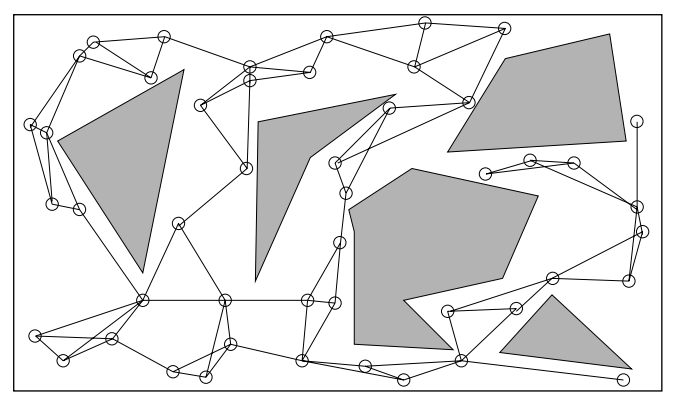
\includegraphics{roadmap}
\centering
\caption{An example of a roadmap }
\label{fig:roadmap_example}
\end{figure}

\subsubsection{Query}
When you have a start point and end point, you connect them to the graph and then using graph searching algorithm to find path from start to end.

\subsubsection{Failure}
Some reasons to failure:
\begin{itemize}
\item Connectivity: disconnected graph
\item Obstacles are very closed to the others. 
\end{itemize}
Solution: generate more samples.\\

\begin{figure}
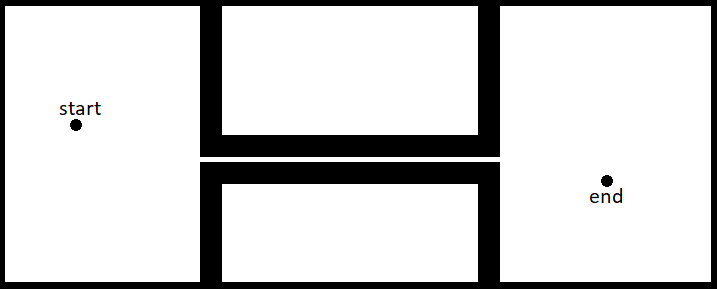
\includegraphics{closed_obs}
\centering
\caption{An example when obstacles are very closed to each other}
\label{fig:closed_obs}
\end{figure}

But in the case when obstacles are closed to the others, the probability to sample between the obstacles is very unlikely. For example, in figure \ref{fig:closed_obs}, the chance to sample points in the narrow road between 2 obstacles is very low. If you keep sampling more points, the graph will become so dense and will take a lot of time to find a path between start and end point.\\
Solution: sample more points toward edges of the obstacles. We can use binary search to find the closest point to the obstacle that's collision-free, and then sample more points near that point. The process of sampling becomes more expensive, but result graph is less dense and faster to compute path.

\subsection{Visibility PRM}

\end{document}